\chapter{Preparation}

%\section{Background}

\section{Graph representational learning}
\label{sec:GRL}

% Formal definition of graph based data

%% Formal definition of a graph

A \emph{graph} can be formally represented as the tuple $\gG(\sV, \sE, \mX)$ where $\sV$ is the set of nodes in the graph, $\sE$ is the set of edges, and $\mX$ is the input features.
Two nodes of the graph, $v_i, v_j \in \sV$, are \emph{connected} if and only if $(v_i, v_j) \in \sE$ and
%, the edge is directed with $v_i$ as the source and $v_j$ as the destination.
%It is possible to associate data with the edges of the graph where $(v_i, v_j, \textbf{e}_{ij}) \in \sE$ represents a connection between $v_i$ and $v_j$ and associated vector $\textbf{e}_{ij}$.
each node, $v_i \in \sV$, has associated data represented by the \emph{feature vector} $\vx_i = \emX_{i,\star}$ the $i^{th}$, row of $\mX$.

The edges can be represented as an \emph{adjacency matrix}, $\mA$, where 

\begin{equation}
    \label{eq:adj}
    \emA_{ij} = \begin{cases}1 &\text{iff $(v_i, v_j) \in \sE$} \\ 0 &\text{otherwise}\end{cases}.
\end{equation}

%This allows the edge information to be utilised by a NN along with the features $\mX$.
Furthermore, each node, $v_i \in \sV$, has \emph{neighbours} which is set of connected nodes,

\begin{equation}
    \label{eq:neighbour}
    \sN_i = \{v_j | (v_i, v_j) \in \sE \vee (v_j, v_i) \in \sE\},
\end{equation}

where each element of $\sN_i$ is considered a \emph{neighbour} of the node $v_i$.
%For ease of writing $\mX_{\sN_i}$ represents the features of the neighbours of $v_i$ defined as 
%\begin{equation}
%    \label{eq:neighbour-reps}
%    \mX_{\sN_i} = \{\{\vx_j | v_j \in \sN_i\}\}.\footnote{As the neighbours may have the same feature vector this must be a multiset.}
%\end{equation}
%If there is data associated with the edges, such as edge weights, this value is stored in the adjacency matrix.
%An unweighted graph can be described as a weighted graph with edge weights of value $1$.
%Adjacency matrices can be very sparse, meaning they have very few non-zero values, and therefore the matrix is commonly stored in a \emph{coordinate matrix} (COO) of size $2 \times N$ for $N$ edges in the graph thus only storing edge information.

% Formal definition of representational learning

The goal of \emph{graph representational learning} is to find, for each $v_i \in \sV$, a vector $\vh_i^{(l)}$ based on the the input features $\mX$ and adjacency matrix $\mA$, where $\vh_i^{(0)} = \vx_i$.
$\vh_i^{(l)}$ is the \emph{node representation} after the $l^{th}$-layer and $\mH^{(l)}$ is the total graph representation where $\mH_{i, \star}^{(l)} = \vh_i^{(l)}$.
%It is therefore important to consider an updated version of equation \ref{eq:neighbour-reps} as $mH_{\sN_i}^{(l)} = \{\{\vh_j^{(l)} | v_j \in \sN_i\}\}$ however $\mX_{\sN_i}$ will be used and the

% Comparison of graph, edge and node based learning

%% Expand the above definition to edges and graphs
%% discussion of edge weights in training when talking about edge learning
%% discussion of pooling functions with graph classification

These representations may then be used as input to a classifier to solve one of 3 different classification tasks: node classification, graph classification, link prediction.
This project focuses on node classification, where each node is assigned a label, and graph classification, where the graph as a whole is assigned a label.
%Node classification classifies each node solely on the final node representation $\vh_i$.
%Comparitively graph classification aggregates all of the node representations and classifies the entire graph accordingly.

\subsection{Graph neural networks}

%% Formal definition of a function on this graph
%%      Think about Petars talk here

%% The idea of invariants, equivariants and approaches

The updated node representations should depend on the local neighbourhood of each node.
If the same local neighbourhood representations were to be permuted the updated representation should remain the same as the neighbourhood topology is the same.
Therefore consider a vector valued function, $\vf$, taking neighbourhood representations, $\mX_{\sN_i}$, and adjacency matrix, $\mA$, and producing a neighbourhood representation $\vf(\mX_{\sN_i}, \mA)$.
Given some permutation, $\mP$, $\vf(\mP\mX_{\sN_i}, \mP\mA\mP^T) \equiv \vf(\mX_{\sN_i}, \mA)$.\footnote{As the rows and columns of the adjacency matrix must be permuted the permutation matrix is applied twice, with the premultiplication transposed to permute the columns.}

Furthermore, if the node features are permutated then the updated node representations should be as well.
Thus consider a matrix-valued function, $F$, taking the input representations and adjacency matrix, and producing a new representation matrix.
It must be the case that $F(\mP\mX, \mP\mA\mP^T) \equiv \mP F(\mX, \mA)$.

For the node representation update function, $F$, to be equivariant it suffices for the neighbourhood representation function to be invariant, \Aref{app:perm}.
For the neighbourhood representation to be invariant an invariant aggregation function, $\bigoplus$, combines updated neighbourhood representations.
Thus a neighbour representation for $\vx_i$ is $\bigoplus_{\vx_j \in \mX_{\sN_i}}c_{ij}\bm{\psi(\vx_j)}$,\footnote{Multiple formulations exist and is an area of active research.}
where $\bm{\psi}$ is a node representation update function.
This leads to a general invariant node representation update function

\begin{equation}
    \label{eq:conv-def}
    \bm{\phi}(\vx_i, \mX_{\sN_i}) = \bm{\varphi}(\vx_i, \bigoplus_{\vx_j \in \mX_{\sN_i}}c_{ij}\bm{\psi}(\vx_j)).
\end{equation}

%This function can be described by a function, $f$, which acts on a single node, $v_i$, using the feature vector, $\vx_i$, and neighbours, $\sN_i$.
%Rather than $f$ being applied to the input features consider some node representation $\vh_i^{(l)}$ after $l$ iterations, where $\vh_i^0 = \vx_i$.
%Then $\vh_i^{(l+1)} = f^{(l)}(\vh_i^{(l)}, \sN_i)$, where $f^{(l)}$ is the $l^{th}$ application of the function $f$.

% Formal definition of a graph neural network

%% Expand on the invariants and equivariants above (maybe only start that here)
%% Formalise the notion of how a GNN would behave
%% Discuss the differing approaches

% Potentially the motivation behind this formalisation

%% This is the invariance and equivariance
%% Might be possible to motivate this from the development perspective

% Identify the root of deep learning in its formulation

%% Highlight the concept of non-linear layers
%% potentially a brief discussion on the importance of this concept

\subsection{Graph convolutional network}
\label{sec:GCN}

% Formal implementation of Graph Convolutional Network

%% Expand on the convolutional approach to discuss this formulation

\subsubsection{As a GNN}

The GCN is the simplest implementation of the formulation outlined above.
The principle is to add the degree-weighted sum of a node's neighbour representations to the current node representation.
%This maintainsd the invariance constraint but nodes with a high degree are overly represented and so each term is normalised by the degree of the connecting nodes.
This results in the common representation of GCN as

\begin{equation}
    \label{eq:GCN-as-GNN}
    f(\vh_i^{(l)}, \mA) = \frac1{d_i + 1}\vh_i^{(l)} + \sum_j^N\frac{\emA_{ij}}{\sqrt{(d_i + 1)(d_j + 1)}}\vh_j^{(l)},
\end{equation}
%\begin{equation}
%    \vh_i^{(l+1)} = \sigma(f(\vh_i^{(l)}, \mA)\theta_i^{(l)})
%\end{equation}

where $d_i = \sum_j^N \emA_{i,j}$ (the degree of node $v_i$), $\theta_i^{(l)}$ is a learnable parameter, and $\sigma$ is an activation function. Comparing to equation \ref{eq:conv-def} $c_{ij} = \frac1{\sqrt{(d_i + 1)(d_j + 1)}}$ and $\sum_j^N$ is equivalent to $\bigoplus_{\vx_j \in \mX_{\sN_i}}$. 

%\begin{align*}
%    &\vx_j \in \mX_{\sN_i} \\
%    \iff &j \in \sN_i &&\text{by def. \ref{eq:neighbour-reps}} \\
%    \iff &(v_i, v_j) \in \sE \vee (v_j, v_i) \in \sE &&\text{by def. \ref{eq:neighbour}} \\
%    \iff &A_{ij} = 1 &&\text{by def. \ref{eq:adj}}
%\end{align*}

%To better demonstrate that the same operation is being applied to each neighbouring representation (including the nodes current representation) 
equation \ref{eq:GCN-as-GNN} may be rewritten as

\begin{equation}
    \label{eq:same-op}
    f(\vh_i^{(l)}, \mA) = (d_i + 1)^{-\frac12}1(d_i + 1)^{-\frac12}\vh_i^{(l)} + \sum_j^N(d_i + 1)^{-\frac12}\emA_{ij}(d_i + 1)^{-\frac12}\vh_j^{(l)}.
\end{equation}

Let $\mD$ be the degree matrix, $\emD_{ii} = \sum_j^N \emA_{ij}$ then
%and $\mH^{(l)}$ the node representations of the graph after layer $l$
equation \ref{eq:same-op} becomes

\begin{equation}
    F(\mH^{(l)}, \mA) = (\mD + \mI)^{-\frac12}(\mA + \mI)(\mD + \mI)^{-\frac12}\mH^{(l)}.
\end{equation}

Let $\widetilde{\mA} = \mA + \mI$, then $\widetilde{\emD}_{ii} = \sum_j^N \widetilde{\emA}_{ij} = \sum_j^N [\emA_{ij} + 1] = \emD_{ii} + 1$ thus $\widetilde{\mD} = \mD + \mI$.
This reformulation gives the following graph operator 
\begin{equation}
    \label{eq:op}
    \mS = \widetilde{\mD}^{-\frac12}\widetilde{\mA}\widetilde{\mD}^{-\frac12}.
\end{equation}

Thus a GCN layer can be interpreted as a graph operator and non-linear activation
\begin{equation}
    \label{eq:GCN1}
    \mH^{(l+1)} = \sigma(\mS\mH^{(l)}\bm{\Theta}^{(l)}).
\end{equation}
%resulting in the following formulation
%\begin{equation}
%    F(\mH^{(l)}, \mA) = \mS\mH.
%\end{equation}

%The function is parameterised by a weight matrix, $\bm{\Theta}$, to give a single layer 

\subsubsection{As a convolution}
\label{sec:conv}

To motivate the idea of the SGC it is important to think of $\mS$ from a different perspective, as a graph convolution filter. A convolution is a multiplication of two functions, in this case a signal,\footnote{The signal is a function $\vh : \sV \to \R^n$, however, the nodes are fixed so define $\vh_i \equiv \vh(v_i)$.}
represented by the node representation $\vh_i \in \R^n$, and a filter, $f_\theta$ paramaterised by $\theta$.

As an analogy to Fourier analysis $f_\theta \star_\sG \vh_i$ is defined in the graph spectral domain.
Any signal on a graph can be projected onto the eigenvectors of the graph Laplacian, $\mL = \mD - \mA = \mU\bm{\Lambda}\mU^T$, where $\bm{\Lambda} = \operatorname{diag}(\lambda_0, ..., \lambda_{n-1})$.
Therefore the graph Fourier transform of a graph function $g$ is
\begin{equation}
    \hat{g} = \mU^Tg
\end{equation}

%As an analogy to classical Fourier analysis the operation is defined in the spectral domain of the graph allowing for the convolution to be a pointwise product.
%
%Let $\mL$ be the graph Laplacian with eigendecomposition $\mU\bm{\Lambda}\mU^T$ where $\bm{\Lambda} = \operatorname{diag}(\lambda_0, ..., \lambda_{n-1})$. Define $\hat{\vh_i}$, the graph Fourier transform of the signal, as
%\begin{equation}
%    \label{eq:graph-fourier}
%    \hat{\vh_i} = \mU^T\vh_i.
%\end{equation}

%Equation \ref{eq:graph-fourier} carries out the dot product between $\vh_i$ and each of the eigenvectors of the graph Laplacian, $\mL$.
%This corresponds to the ``frequency'' of the signal $\vh_i$ with respect to the frequencies of the graph.
%This transforms $\vh_i$ into its frequency components according to the spectral domain of the graph.

This transformation is applied to $\vh_i$ and $f_\theta$ so that $\hat\vh_i$ and $\hat f_\theta$ are projected onto the graph eigenvectors.
As the graph Laplacian is symmetric the inverse transform exists, applying $\mU$ instead of $\mU^T$.
Thus the graph convolution is defined as $f_\theta \star_\sG \vh_i = \mU(\hat f_\theta \odot \hat\vh_i)$ where $\odot$ is the hadamard product.
To simplifying the calculation let $\hat\mF_\theta = \operatorname{diag}(f_\theta)$,
\begin{equation}
    \label{eq:conv}
    f_\theta \star_\sG \vh_i = \mU\hat\mF_\theta\mU^T\vh_i.
\end{equation}

%followed by an inverse graph Fourier transform. To simplify the equation define 
%\begin{equation}
%    \label{eq:filter1}
%    \hat\mF_{\bm{\theta}} = \operatorname{diag}\hat f_\theta = \operatorname{diag}{\bm{\theta}}
%\end{equation}
%where $\bm{\theta}$ is a vector of parameters which can be learnt by a NN. Resulting in the following formalisation of a graph convolution
%\begin{equation}
%    \label{eq:graph-conv}
%    f_\theta *_\sG \vh_i = \mU\hat\mF_{\bm{\theta}}\mU^T\vh_i.
%\end{equation}

To prevent $\hat\mF_\theta$ growing with the dimension of the signal it can be defined as a power series of the fixed Laplacian eigenvalue matrix,
\begin{equation}
    \label{eq:filter}
    \hat\mF_{\bm{\theta}} = \sum_{j=0}^k\theta_j\bm{\Lambda}^j.
\end{equation}

%\textit{Kipf et al.}~\cite{kipf2016semi} suggest using $k=1$ and define $\theta = \theta_0 = -\theta_1$ resulting in
Using this new filter in equation \ref{eq:conv} yields the following formulation of the graph convolution
\begin{equation}
    \label{eq:GCN-comp}
    f_\theta *_\sG \vh_i = \sum_{j=0}^1\theta_j(\mU\bm{\Lambda}\mU^T)^j\vh_i.\footnote{$\mU\bm{\Lambda}^j\mU^T = \mU\underbrace{\bm{\Lambda}\cdots\bm{\Lambda}}_j\mU^T = \underbrace{\mU\bm{\Lambda}\mU^T\mU\cdots\mU^T\mU\bm{\Lambda}\mU^T}_j = (\mU\bm{\Lambda}\mU^T)^j$}
    %= \theta(\mI - \mL)\vh_i.
\end{equation}

Computation of the eigendecomposition of $\mL$ is expensive for large graphs so \textit{Hammond et al.}~\cite{hammond2011wavelets} suggest using Chebyshev polynomials (\Aref{app:chebyshev}).
%With the additional assumption that a NN can adapt to scaling we assume that the maximum eigenvalue is approximately $2$.
Using the first order Chebyshev polynomial, $\mI + (\mL - \mI)$, and the normalised graph Laplacian, $\mL^{sym} = \mD^{-\frac12}\mL\mD^{-\frac12} = \mI - \mD^{-\frac12}\mA\mD^{-\frac12}$ equation \ref{eq:GCN-comp} can be written as 
\begin{equation}
    \label{eq:no-norm}
    f_\theta *_\sG \vh_i \approx (\theta_1\mI + \theta_2(\mL - \mI))\vh_i \approx \theta(\mI + \mD^{-\frac12}\mA\mD^{-\frac12})\vh_i,
\end{equation}

where $\theta = \theta_1 = - \theta_2$ as suggested by \textit{Kipf et al.}~\cite{kipf2016semi}.
The filter can then be used to update the node representations as such
%Applying an individual paramaterised filter to each signal, that is each node, in the graph results in the following formulisation
\begin{equation}
    \label{eq:GCN2}
    \mH^{(l+1)} = \sigma((\mI + \mD^{-\frac12}\mA\mD^{-\frac12})\mH^{(l)}\bm{\Theta}^{(l)})
\end{equation}

To reduce the size of eigenvalues, and thus vanishing/exploding gradients, \textit{Kipf et al.}~\cite{kipf2016semi} apply the following renormalisation to equation \ref{eq:no-norm} 
\begin{equation}
    \label{eq:norm}
    \mI + \mD^{-\frac12}\mA\mD^{-\frac12} \to \widetilde{\mD}^{-\frac12}\widetilde{\mA}\widetilde{\mD}^{-\frac12} = \mS.
\end{equation}

This renormalisation matches the graph operator in equation \ref{eq:op} demonstrating that GCN behaves as a graph filter.
If either formulation is used for node classification a linear classifier is appended to the computation resulting in 
\begin{equation}
    \label{eq:cls}
    \hat\mY = \operatorname{softmax}(\mS\mH^{(k-1)}\bm{\Theta}^{(k)}).
\end{equation}


%= \widetilde{\textbf{D}}^{-\frac12}\widetilde{\mA}\widetilde{\textbf{D}}^{-\frac12}\mX\textbf{\Theta}$

% Link to the paper

%% Lay out the exact formulation from the paper
%% Explain this formulation
%% include the motivations/reasonings from the paper

% Discussion of importance in the field?

%% Description of the fact that this is the first graph approach
%% Maybe a link to DeepSet

\subsection{Simplified graph convolution}
\label{sec:SGC}

% Motivation behind SGC

%% Reiterate the points made in the introduction
%% Now specifically highlight these areas in the GCN formulisation

As both approaches in \Sref{sec:GCN} demonstrate a GCN can be broken down into individual layers, containing a linear graph operation, stacked together using a non-linear activation function.
This means that the $k^{th}$-layer node representation requires the calculation of all the non-linear activations up until $k$.
%This is apparent when looking at the formulation in equation \ref{eq:GCN1}.

\paragraph{Linearization.}
Considering the linear graph operation as a spectral filter as described in equation \ref{eq:norm} the non-linearity between layers may be considered non-critical to GCN performance.
Instead, the benefit comes from the local averaging from successive filter applications as hypothesised by \textit{Wu et al.}.
%\textit{Wu et al.}~\cite{wu2019simplifying} consider this hypothesis citing the benefit arises from the local averaging as apparent in the graph operation formulation described in \Sref{sec:conv}.
%The resulting model is therefore a linear multiplication of the normalised spectral filters and parameter matrix.
Removing the non-linear activation functions from equation \ref{eq:cls} results in
\begin{equation}
    \hat\mY = \operatorname{softmax}(\underbrace{\mS\cdots\mS}_k\mX\underbrace{\bm{\Theta}^{(1)}\cdots\bm{\Theta}^{(k)}}_k),
\end{equation}

where the filter is applied $k$ times to allow for the retention of the receptive field.
As $\bm{\Theta}^{(i)}$ is a learnable parameter the model may instead learn a single parameter
\begin{equation}
    \label{eq:theta}
    \bm{\Theta} = \underbrace{\bm{\Theta}^{(1)}\cdots\bm{\Theta}^{(k)}}_k.
\end{equation}

Thus the final model becomes
\begin{equation}
    \hat\mY = \operatorname{softmax}(\mS^{k}\mX\bm{\Theta}).
\end{equation}

As $\mS$ is fixed for a specific graph $\mS^k\mX$ is fixed if $\mX$ is fixed.
Thus SGC can be broken down into representation extraction, $\bar\mX = \mS^k\mX$, and a classification
\begin{equation}
    \label{eq:SGC}
    \hat\mY = \operatorname{softmax}(\bar\mX\bm{\Theta}).
\end{equation}
This allows for $\bar\mX$ to be precomputed for given node features $\mX$.
%or just $\mS^k$, allowing for the pre-computation of different node features.
%Furthermore, different node features can be quickly calculated as $\mS^k$ can be precomputed.

Rather than considering how many layers an SGC model has the equivalent notion of \emph{degree} is used where the degree is the power of $\mS$.
This directly corresponds to the receptive field of the model where a $k$-degree SGC model has the same receptive field as a $k$-layer GCN model.

\paragraph{Drawbacks}
SGC suffers from vanishing/exploding values in $\bm{\Theta}$ and over-smoothing\footnote{where the node representations become increasingly uniform as the increased receptive field of the model results in a global averaging of the nodes of the graph.}.
SGC has a fixed feature extraction step preventing influence on intermediate node representations.
These drawbacks motivate the extensions presented in \Sref{sec:extensions-imp} and \Sref{sec:extension-eval}.

%The fomulation in equation \ref{GCN-as-GNN} highlights that at after each layer each node representation includes a representation of its immediate neighbours.
%This means that the $k^{th}$-layer node representations are influenced by the node representations at most $k$-hops away. 

% Demonstration of how the GCN leads to the SGC

%% Demonstrate that the removal of layers logically leads to SGC
%% Explanation of how the weight matrix would behave
%% Potential hint or discussion about the effect of weight decay later

\section{Explainability}

% Overview of the concept of explainability

%% This needs some proper reading in the topic see below

% This probably requires reading some papers "yay"

NNs are presented as black-box models where the decision process used to infer an output based on input is opaque to a user.
This results in mistrust in NNs especially deep NNs where the relationship between input and output is complex.

The goal of explainability is to provide a human interpretable representation of the model's decision process.
Ideally, global explanations are provided allowing insight into the model's full decision process rather than a local feature.

The proposed approach to explainability that this dissertation follows is that of concepts as these can be inferred after training and thus do not affect model performance.
As GNNs utilise both graph structure and node features concepts can provide a human interpretable representation of a GNNs decision process.

\subsection{Concepts}
\fig{concept-2}{A graph concept from BA Shapes demonstrating the desired properties of meaningfulness, coherency and importance. Green highlights the node of interest and pink represents the local neighbourhood.}

% Explanation of what a concept is generally

%% Again this requires proper reading in the subject see above

A concept is a high-level unit of information that is more interpretable than standard input units such as individual pixels or characters.
A precise definition of a concept in the general sense is hard to formalise so \textit{Ghorbani et al.}~\cite{ghorbani2019towards} propose the following desired properties
\begin{itemize}
    \item[]
        \smalltitle{Meaningfulness}
        dictates that the concept is semantically meaningful on its own requiring no additional information to provide semantic meaning.
        For example, ``Apple'' or ``Personal Pronoun'' rather than an individual pixel or character.
        This is seen in figure \ref{fig:concept-2} as all the graphs can be interpreted as abstract houses.
    \item[]
        \smalltitle{Coherency}
        requires examples within a concept to be perceptually the same as each other whilst simultaneously being different from examples within other concepts.
        This can be further constrained to require identical examples.
        For example, ``Stripes'' should contain examples of stripes and no examples of circles, if ``Circles'' is another concept.
        This is seen in figure \ref{fig:concept-2} as all the graphs are isomorphic and only highlight the ``roof''.
    \item[]
        \smalltitle{Importance}
        represents how necessary the presence of a concept is to the prediction of a class.
        For example, the classification of a specific object requires that the object's concept to be present but no need for background concepts.
        This is seen in figure \ref{fig:concept-2} as the idea of a house is necessary to know whether the highlighted node is a ``roof''.
\end{itemize}

% Relating the explanation to graph based Datasets

%% Demonstrate the idea of concepts translates to subgraphs
%% Focus on the node classification task for this explanation
%% Potentially a motivating example

\paragraph{Graph concepts} can therefore be described by exemplar subgraphs of the input graph.
These subgraphs represent both the structure and the node features defining the properties of a concept.
The graph concepts satisfy the above desiderata: meaningfulness relates to the size of the subgraph, coherency relates to subgraph isomorphy, and importance relates to classification based on subgraphs alone.
Figure \ref{fig:concept-2} is an example graph concept created using the techniques in \Sref{sec:GCE}.

% Discussion of complications when looking at graph classification

%% Identify the issue when scaling to graph classification
%% Discuss solutions and the chosen solution for this project

\subsection{Graph concept explainer}
\label{sec:GCE}

% The motivation for the paper

%% The human in the loop aspect of this project
%% Link in ideas from GNNExplainer

\emph{Graph concept explainer} (GCExplainer) proposed by \textit{Magister et al.}~\cite{magister2021gcexplainer} focuses on unsupervised concept extraction with human input to achieve meaningfulness and coherency.
GCExplainer automates concept extraction by clustering the node representations of a GNN model and mapping each cluster to a concept.
The aim is to provide global explanations for a specific dataset class to better understand how a GNN model operates.

% Discussion of the metrics

%% Formulisation of the two metrics that are presented
%% Discussion what each metric measures with link to results
%% Discussion of short comings of clusterings
%% Discussion of further benefits of latent space

\paragraph{Concept extraction}
uses $k$-Means clustering on the node representations of the final GNN layer as recommended by \textit{Magister et al.}~\cite{magister2021gcexplainer}.
This clusters the input graph's nodes by the similarity of the representations as the model will treat a cluster's nodes the same.
Subgraphs centred on a cluster's nodes provide the high-level unit required by \textit{Ghorbani et al.}~\cite{ghorbani2019towards}.
An example of an extracted concept is presented in figure \ref{fig:concept-2}.
%For the purposes of SGC the same process is carried out on $\bar\mX$, the pre-computed features.

\paragraph{Concept scores} are generated for each concept representing how meaningful, coherent and important a specific set of concepts are.
These scores allow for further exploration of the concept space for a specific model.

\paragraph{Concept purity}
relates to the coherence of a concept and is best represented by subgraph isomorphy.
High concept purity indicates a coherent concept and therefore a global concept of the model.
As concept purity is tied to graph similarity \textit{Magister et al.}~\cite{magister2021gcexplainer} suggest using the \emph{graph edit distance} (GED) which calculated as 
\begin{equation}
    \label{eq:GED}
    \operatorname{GED}(\sG_1, \sG_2) = \underset{e_i,...,e_k \in \gamma(\sG_1, \sG_2)}{\operatorname{min}} \sum_{i=1}^{k}c(e_i)
\end{equation}
where $\gamma(\sG_1, \sG_2)$ is the set of edits to transform $\sG_1$ into $\sG_2$ and $c(e_i)$ is the cost of carrying out an edit operation $e_i$.\footnote{This process is NP-Hard and so in most cases an exact purity score is infeasible to compute.}
A high purity score is represented by a lower number with 0 being completely pure.
The concept in figure \ref{fig:concept-2} has a purity score of 0 as all the graphs are isomorphic.

\paragraph{Concept completeness}
relates to the importance of the concept determining whether the correct output can be predicted from the concepts alone.
High accuracy in classifying the graph according to its concepts indicates that the concepts extracted are important.
As the concept space is not easily separable by classifiers such as logistic regressors \textit{Magister et al.}~\cite{magister2021gcexplainer} suggest using a decision tree\cite{kazhdan2020now}.

% Detailing why this method was chosen

%% The improvements seen in the paper in regards to visual comparison
%% The clear metrics for comparison

\paragraph{Comparing concepts} between two models trained on the same dataset can give an indication as to how the two models differ in their inference.
Furthermore, the differences present between the two models provide further insight into how the model reason.
Therefore, the described process of concept extraction and evaluation is used in comparing how SGC and GCN operate to analyse the importance of non-linearity in GNNs.  

\section{Datasets}
\label{sec:datasets-theory}

% Continue the concepts in GRL subchapter
% There may be more details about implementation
% May need chapters here or somewhere else about inductive v. transductive!!

To evaluate different GNN models using the metrics described in \Sref{sec:GCE} a trained model is evaluated on specific graph data and concepts extracted from the result.
%To train the model the a notion of a graph dataset needs to be defined.
As described in \Sref{sec:GRL} there are two different classification tasks of interest:
Node classification datasets, assigning a class to each node, and graph classification datasets, assigning a class to the entire graph.
A graph dataset is therefore described by a collection of graphs and corresponding class labels.

Node classification datasets generally include a single \emph{connected} graph where at least one path from every node to every other node exists.
In comparison, graph classification tasks include a set of different graphs with a range of topologies.
These differences give rise to the notion of transductive and inductive learning, \Aref{app:datasets}.

\subsection{Synthetic datasets}
\label{sec:synth}

% From GRL and the overview discuss a bottom up approach
% Discuss how certain properties can be instilled
% Relation to graph theory or importance thereof

To better analyse concepts it is easier to construct graphs with specific properties that produce interpretable concepts.
Because these graphs are generated based on desired properties they are considered synthetic graphs.
To carry out the analysis of the concept extraction and evaluation described in \Sref{sec:GCE} the five synthetic graphs presented by \textit{Ying et al.}~\cite{ying2019gnnexplainer} are used.

The construction of these graphs includes a base graph onto which multiple copies of the same \emph{motif} are attached.
A motif is a simple graph structure that should be easily recognised by a GNN and is human-interpretable.
The motifs and base graph have different labels and the goal is to classify each node according to the graph structure the node is a part of.
%Note that the class of a node is dependent on the structure the node is part of rather than the features of the nodes.

\paragraph{Motifs}
\begin{table}
    \centering
    \begin{tabular}{cccc}
        \textbf{Shape (House)} &
        \textbf{Community} &
        \textbf{Grid} &
        \textbf{Cycle}\\
        \midrule
        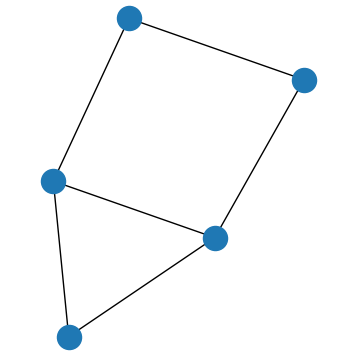
\includegraphics[width=0.2\textwidth]{figures/house.png} &
        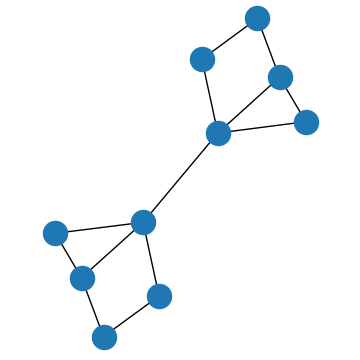
\includegraphics[width=0.2\textwidth]{figures/community.png} &
        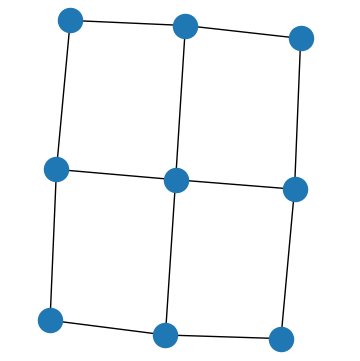
\includegraphics[width=0.2\textwidth]{figures/grid.png} &
        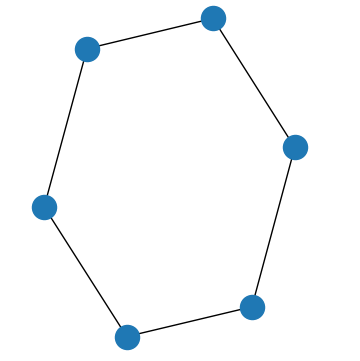
\includegraphics[width=0.2\textwidth]{figures/cycle.png} \\
    \end{tabular}
    \caption{The four different motifs used by the synthetic datasets. Each motif is attached to a specific base graph. Note that the community motif is created by combining two different shape motif graphs.}
    \label{tab:motifs}
\end{table}


are highly ordered graph structures that are easy to identify and differ from the structure of the base graph.
The four motifs can be seen in figure \ref{tab:motifs}.
As these motifs are also very simple they speed up the intensive process of calculating concept purity.

The following graphs are used as base graphs:

\paragraph{Barabasi-Albert (BA)}
a densely connected graph where nodes are probabilistically connected to each other.
The probability of a node connecting to another is proportional to the degree of the node thus creating hubs of densely connected nodes.

\paragraph{Tree}
a binary symmetric tree (BST) as this is very sparse in comparison to Barabasi.
These two base graphs provide two different scenarios to compare a model's ability to identify the motifs accurately.

Not all motifs and base graphs are paired together and only BA Shapes\footnote{Which utilises the house motif}, BA Grid, Tree Grid and Tree Cycles are considered.
BA Community combines two BA Shapes graphs and requires distinguishing between the communities.
All datasets have no discerning node features except for BA Community which distinguishes between communities.

\subsection{Real-world datasets}
\label{sec:RWD}

% Linking to motivation and GRL
% Demonstrating that these techniques are important for real world use
% Discussions of the short comings of this approach

\textit{Wu et al.}~\cite{wu2019simplifying} evaluate the performance of SGC on a variety of datasets including Cora, Citeseer and PubMed\cite{citation}.
%These three datasets match the size of the datasets that are used in \textit{Magister et al.} and therefore are used for results reproduction.
Each graph represents a citation network where nodes are articles and edges are citations.
The node features are bag-of-word embeddings generated from the article text.
These datasets are available through \texttt{PyTorch Geometric}~\cite{Fey/Lenssen/2019} under the Planetoid\cite{planetoid} datasets.

To produce meaningful results that reflect real-world applications of GNNs two real-world datasets are used.
These two datasets are graph classification datasets and therefore inductive datasets compared to the transductive synthetic datasets.
These datasets are part of TUDataset~\cite{Morris+2020} available through \texttt{PyTorch Geometric}\cite{Fey/Lenssen/2019}.

\paragraph{REDDIT BINARY}
is a dataset where each graph represents a discussion on Reddit with users as nodes and comments as edges.
The discussions are sampled from IAmA, AskReddit, TrollXChromosomes, and atheism.
The task is to classify the graphs as question-answer or discussion threads.

\paragraph{Mutagenicity}
is a dataset where each graph is a chemical compound where nodes are atoms and edges are chemical bonds.
The chemical compounds correspond to drugs some of which are mutagens and the rest are not.
The task is to classify the graphs as to whether or not they are mutagens.

\section{Tools used}

% I believe this is stuff like vim
% Pytorch, pytorch lightning and pytorch geometric
% scipy and numpy
% python unittest and typing
% python linter through vim

\paragraph{Programming languages}
I use Python to write the majority of the software as there is a lot of existing support for machine learning frameworks.
Furthermore, Python is easy to read, debug and experiment with which is useful for developing new models.

To reduce the need for human input when running multiple experiments to get confidence intervals or hyperparameter tuning dynamically generated bash scripts were used.
To allow for easier reproducibility and iteration I utilise YAML files to store build configurations for all of my models.

\paragraph{Software development}

A personal configuration of \texttt{NeoVim} was used to develop the code as this has high customizability allowing personalised linters.
Additionally, local \texttt{Tensorboard}~\cite{tensorflow2015-whitepaper} instances help visualise and analyse the progress of experiments in realtime, \texttt{Git} and \texttt{Github} implement version control with \texttt{scp} and the \texttt{Student Run Computing Facility} as a third backup for experiment results.
\texttt{Google Colab} was occasionally used for compute units to run the large experiment batches.

\paragraph{Libraries}
\label{sec:libraries}

The major libraries used where \texttt{PyTorch}~\cite{paszke2019pytorch} and \texttt{PyTorch Geometric}\cite{Fey/Lenssen/2019} an extension to \texttt{PyTorch} which includes support for GRL.
\texttt{PyTorch} was chosen over \texttt{Tensorflow}~\cite{tensorflow2015-whitepaper} as it is more ``pythonic'' and \texttt{PyTorch Geometric} is a simpler framework to use.
To help with running experiments, logging results and reproducibility I use \texttt{Lightning AI} which handles the underlying training and testing loop with Tensorboard support.
\texttt{Hyperopt}~\cite{bergstra2013making} is also used as \textit{Wu et al.}\cite{wu2019simplifying} state this method was used to find the weight decay hyperparameter.

For scientific computing when analysing concepts I use \texttt{Numpy} and \texttt{scikit-learn}~\cite{scikit-learn}. For the visualisation of graphs I use \texttt{NetworkX}\cite{SciPyProceedings_11} to draw the graphs and \texttt{Matplotlib}\cite{Hunter:2007} to visualise the result and hyperparameter surfaces. \texttt{NetworkX} is included in the \texttt{PyTorch Geometric} library.

For unit tests I use Python's own \texttt{unittest} library and to help with software development I use Python's \texttt{typing} library alongside the built-in typing functionality of the other libraries. Additionally, I use \texttt{tqdm}~\cite{casper_da_costa_luis_2023_7697295} to visualise progress during concept analysis.

\section{Requirements analysis}

% definitely think this is useful
% to be figured out later

The success criteria of the project proposal (\Aref{ch:proposal}) define three main stages of development each requiring individual and joint requirements.
Further requirements include improving the reproducibility of the code and results with additional requirements for extensions.

Table \ref{tab:requirements} demonstrates the requirements analysis for this project.
Risk represents how critical a requirement's success is given how difficult it will be to implement.

``-'' represents a general requirement for the project to be implemented, ``S'' represents a requirement based on the given success criteria, and ``E'' represents a requirement that is an extension to the core project.

\begin{table}
    \centering
    \begin{tabular}{p{0.11\textwidth}|p{0.5\textwidth}|p{0.15\textwidth}|p{0.11\textwidth}}
        \multicolumn{1}{c}{\textbf{Source}} &
        \multicolumn{1}{c}{\textbf{Requirement}} &
        \multicolumn{1}{c}{\textbf{Importance}} &
        \multicolumn{1}{c}{\textbf{Risk}} \\ 
        \midrule
        - & Download Planetoid and TUDatasets & \hlc[red!50]{Essential} & \hlc[green!50]{Low} \\
        - & Build synthetic datasets & \hlc[red!50]{Essential} & \hlc[red!50]{High} \\
        - & Implement ML pipeline & \hlc[red!50]{Essential} & \hlc[orange!50]{Medium} \\
        - & Create model configuration format & \hlc[orange!50]{Preferrable} & \hlc[green!50]{Low} \\
        S1 & Implementation of SGC & \hlc[red!50]{Essential} & \hlc[orange!50]{Medium} \\
        S1 & Implement Hyperparameter sweep framework & \hlc[orange!50]{Preferrable} & \hlc[green!50]{Low} \\
        S1 & Hyperparameter sweep for SGC\tablefootnote{GCN hyperparameters should be sufficient for a well performing SGC model, but for true comparison a full sweep of reasonable parameters should be made.} & \hlc[orange!50]{Preferrable} & \hlc[green!50]{Low} \\
        S2 & Implementation of GCN & \hlc[red!50]{Essential} & \hlc[green!50]{Low} \\
        S1, S2 & Match prior performance & \hlc[red!50]{Essential} & \hlc[red!50]{High} \\
        S1, S2 & Implement model hooks to extract activation space & \hlc[red!50]{Essential} & \hlc[green!50]{Low} \\
        S1, S2 & Implement clustering for concept extraction & \hlc[red!50]{Essential} & \hlc[green!50]{Low} \\
        S3 & Implementation of concept purity & \hlc[red!50]{Essential} & \hlc[green!50]{Low} \\
        S3 & Implementation of concept completeness & \hlc[red!50]{Essential} & \hlc[orange!50]{Medium} \\
        S1, S2, S3 & Concept visualisation & \hlc[orange!50]{Preferrable} & \hlc[green!50]{Low} \\
        E & Extend SGC to graph classification & \hlc[green!50]{Optional} & \hlc[orange!50]{Medium} \\
        E & Improve performance of SGC & \hlc[green!50]{Optional} & \hlc[gray!50]{Unknown} \\
        E & Combine SGC and GCN & \hlc[green!50]{Optional} & \hlc[gray!50]{Unknown} \\
        E & Latent space comparison of GCN and SGC & \hlc[green!50]{Optional} & \hlc[gray!50]{Unknown} \\
    \end{tabular}
    \caption{Requirements analysis for the project.}
    \label{tab:requirements}
\end{table}

%\begin{enumerate}
%    \item[S1] Implementation of SGC
%    \item[S2] Implementation of GCN
%    \item[S3] Implementation of concept evaluation
%\end{enumerate}



\section{Software methodology}

% Generally waterfall approach to design
% But iterative when looking at the results and direction forward
% sprint work style between meetings

For the core of my project I adopt a Waterfall method~\cite{royce1970managing} for the project:

\begin{equation*}
    \textit{Requirements analysis} \longrightarrow \textit{Design} \longrightarrow \textit{Implementation} \longrightarrow \textit{Testing} \longrightarrow \textit{Evaluation}
\end{equation*}

During the \textit{Design} phase I start with a skeleton implementation of the ML pipeline and focus on each of the requirements in turn carrying out both \texttt{Implementation} and \texttt{Testing} together where possible.
At each stage I confirm that the implemented requirement integrates with the rest of the project using dummy data if a module is not implemented.
The \textit{Evaluation} stage includes all the experiment runs and concept analysis required to meet my success criteria replacing \textit{Operations} which is not required for my project.

My extensions do not fit into the Waterfall method as they are research-based in nature. Therefore, I switch to an Agile software development~\cite{beck2001manifesto} to allow the project to adjust to the experimental results achieved during development.

\section{Testing}
\label{sec:testing}

% unittest for specific sections of code and infrastructure
% comparison to paper baselines when dealing with model implementation

Machine learning does not provide a precise metric against which the correctness of an implementation can be verified.
This is due to the factors that contribute to a machine learning model's performance such as hyperparameters, initialisation/random seeds, architecture and dataset.
As an example a trained model may result in poor results because the underlying architecture is not suited to the dataset, there is too much noise in the data, or there is a software bug.
Thus, unlike traditional software development, it is harder to verify that an ML model or algorithm has been implemented correctly.
However, my project does include software that follows traditional software development and therefore use the following two testing approaches:

\paragraph{Unit testing}
is suitable for traditional software development where a specific result is required for specific input.
Concept analysis and dataset handling fall into this category.
These two aspects are therefore verified using unit testing described in \Sref{sec:testing-imp}.

\paragraph{Reproduction of prior results}
The two main models I use, GCN and SGC, directly follow implementations of the work by \textit{Kipf et al.}~\cite{kipf2016semi} and \textit{Wu et al.}\cite{wu2019simplifying}.
The hyperparameters for the GCN model baseline are available in \textit{Magister et al.}~\cite{magister2021gcexplainer} where accuracy scores are also published.
In \Sref{sec:reproduction} I reproduce the experiment results to verify my ML pipeline, NN implementations and dataset integration.

\section{Licensing}
%%\begin{table}
    \centering
    \begin{tabular}{cc}
        \multicolumn{1}{c}{\textbf{Software dependency}} &
        \multicolumn{1}{c}{\textbf{License}} \\ 
        \midrule
        NumPy & \multirow{5}{*}{3-clause BSD} \\
        scikit-learn & \\
        NetworkX & \\
        PyTorch & \\
        hyperopt \tablefootnote{The license is unnamed but matches the 3-clause BSD license verbatim.} & \\
        \rowcolor{gray!20} tensorboard & \\
        \rowcolor{gray!20} Lightning AI &  \multirow{-2}{*}{Apache 2.0}\\
        matplotlib & \\
        Python & \multirow{-2}{*}{PSFL}\\
        \rowcolor{gray!20}
        PyTorch Geometric & \\
        \rowcolor{gray!20}
        tqdm & \multirow{-2}{*}{MIT} \\
        tqdm & MPL\tablefootnote{tqdm is distributed under both licenses.} \\
    \end{tabular}
    \caption{Licenses for the project dependencies}
    \label{tab:licensing}
\end{table}

\begin{table}
    \centering
    \begin{tabular}{cc}
        \multicolumn{1}{c}{\textbf{Software dependency}} &
        \multicolumn{1}{c}{\textbf{License}} \\ 
        \midrule
        NumPy & \multirow{5}{*}{3-clause BSD} \\
        scikit-learn & \\
        NetworkX & \\
        PyTorch & \\
        hyperopt \tablefootnote{The license is unnamed but matches the 3-clause BSD license verbatim.} & \\
        \rowcolor{gray!20} tensorboard & \\
        \rowcolor{gray!20} Lightning AI &  \multirow{-2}{*}{Apache 2.0}\\
        matplotlib & \\
        Python & \multirow{-2}{*}{PSFL}\\
        \rowcolor{gray!20}
        PyTorch Geometric & \\
        \rowcolor{gray!20}
        tqdm & \multirow{-2}{*}{MIT} \\
        tqdm & MPL\tablefootnote{tqdm is distributed under both licenses.} \\
    \end{tabular}
    \caption{Licenses for the project dependencies}
    \label{tab:licensing}
\end{table}

Table \ref{tab:licensing} includes information about the specific licenses for the project's software dependencies.

All software dependencies used in my project are under permissive licenses allowing me to use the code with no restrictions.
Furthermore, I am free to use the Planetoid~\cite{planetoid} and TUDataset \cite{Morris+2020} datasets available in \texttt{PyTorch Geometric}\cite{Fey/Lenssen/2019} library.
Though some licenses have additional restrictions on source code modification and/or redistribution my project does neither of these actions and only uses the libraries as is.

I license my source code under the MIT license to support further developers and researchers.
This licensing complies with the licenses of my dependencies.

% Definitely need to research this aspect

\section{Starting point}

I have worked with \texttt{PyTorch}~\cite{paszke2019pytorch} and \texttt{PyTorch Geometric}\cite{Fey/Lenssen/2019} and have experience building graph datasets and GNN models.
I use the \texttt{PyTorch Geometric}~\cite{Fey/Lenssen/2019} implementation of GCN layers to build the GCN network, as this is just a baseline model. I also rely on the libraries discussed in \Sref{sec:libraries}.
Aside from these dependencies, I built the project from scratch.

% Discussion of summer project using the same rough build environment
